% !TeX root = ../tesis.tex


\section{Relaciones de Kramers-Kronig}
\label{section:yth}

El estudio experimental de las propiedades ópticas lineales no siempre permite determinar por completo las características ópticas de una muestra \cite{KramersKronigRelationsSum2005}. No obstante, el principio de causalidad en la respuesta óptica de cualquier material permite extraer información adicional a partir de los datos experimentales \cite{KramersKronigRelationsSum2005}.  A partir de la aplicación del principio de causalidad y de la analiticidad de una función óptica lineal compleja, como la susceptibilidad, la función dieléctrica, el índice de refracción o la reflectividad, se deducen las relaciones de Kramers-Kronig (KK), las cuales describen la conexión entre las partes real e imaginaria de una función óptica lineal compleja \cite{KramersKronigRelationsSum2005}. Para deducir las relaciones de KK se considera un material homogéneo e isótropo caracterizado por una función óptica lineal compleja, que en este caso será la función dieléctrica, así como un espacio de frecuencias complejo.

La transformada de Fourier temporal para $\vb{D}$ está dada por~\cite{jacksonClassicalElectrodynamics2021a}
%
\begin{equation}
	\vb{D}(\vb{r},\omega)=\int_{-\infty}^{\infty}\vb{D}(\vb{r},t')e^{i\omega t'}\text{d}t',\label{eq:TFI}
\end{equation}
%
mientras que la transformada de Fourier inversa es
%
\begin{equation}
	\vb{D}(\vb{r},t)=\frac{1}{2\pi}\int_{-\infty}^{\infty}\vb{D}(\vb{r},\omega)e^{-i\omega t}\text{d}\omega.\label{eq:TF}
\end{equation}
%
Al sustituir la Ec. \eqref{eq:d3} en la Ec. \eqref{eq:TF}, se obtiene
%
\begin{equation}
	\vb{D}(\vb{r},t)=\frac{1}{2\pi}\int_{-\infty}^{\infty}\varepsilon(\omega)\vb{E}(\vb{r},\omega)e^{-i\omega t}\text{d}\omega,\label{eq:TF_D_intermedia_1}
\end{equation}
%
y al sustituir la transformada de Fourier de $\vb{E}(\vb{r},t)$, se tiene que
%
\begin{equation}
	\vb{D}(\vb{r},t)=\frac{1}{2\pi}\int_{-\infty}^{\infty}\varepsilon(\omega)e^{-i\omega t}\text{d}\omega\int_{-\infty}^{\infty}e^{i\omega t'}\vb{E}(\vb{r},t')\text{d}t'.\label{eq:TF_D_intermedia_2}
\end{equation}
%
Considerando que los órdenes de integración se pueden intercambiar, dado que la integración se realiza en el mismo intervalo ($-\infty$, $\infty$), la Ec. \eqref{eq:TF_D_intermedia_2} se reescribe como
%
\begin{tcolorbox}[ams align]
	\vb{D}(\vb{r},t)=\frac{1}{2\pi}\int_{-\infty}^{\infty}\int_{-\infty}^{\infty}\varepsilon(\omega)\vb{E}(\vb{r},t') e^{i\omega (t-t')} \text{d}\omega \text{d}t'.\label{eq:TF_D_intermedia_3} 
\end{tcolorbox}
%
\noindent Al realizar el cambio de variable $\tau = t - t'$ y emplear la función constante\footnote{$\delta(\tau)$ es la función delta de Dirac, que cumple con $\int_{-\infty}^{\infty}f(\tau)\delta(\tau)\text{d}\tau=f(0)$ \cite{arfkenMathematicalMethodsPhysicists2011a}.}
\begin{equation}
	\mathcal{F}[1]=\int_{-\infty}^{\infty}e^{-i\omega\tau}=\delta(\tau),
\end{equation}
se reescribe al campo eléctrico como
\begin{equation}
	\vb{E}(\vb{r},t)=\int_{-\infty}^{\infty}\vb{E}(\vb{r},t-\tau)\delta(\tau)=\frac{1}{2\pi}\int_{-\infty}^{\infty}\int_{-\infty}^{\infty}\vb{E}(\vb{r},t-\tau)e^{-i\omega\tau}\text{d}\omega\text{d}\tau.
\end{equation}
%
De forma que al sumar $\vb{E}(\vb{r},t')-\vb{E}(\vb{r},t')$ y multiplicar por $\varepsilon_0/\varepsilon_0$ a la Ec. \eqref{eq:TF_D_intermedia_2}, simplificando se obtiene
%
\begin{equation}
	\vb{D}(\vb{r},t)=\varepsilon_0\left[\vb{E}(\vb{r},t)+\int_{-\infty}^{\infty}G(\tau)\vb{E}(\vb{r},t-\tau)\text{d}\tau\right],\label{eq:TF_D_final} 
\end{equation}
%
\noindent donde $G(\tau)$ es \cite{jacksonClassicalElectrodynamics2021a}
%
\begin{equation}
	G(\tau)=\frac{1}{2\pi}\int_{-\infty}^{\infty}\left[\frac{\varepsilon(\omega)}{\varepsilon_0}-1\right]e^{-i\omega\tau}\text{d}\omega,
	\label{eq:G_tdependent} 
\end{equation}
%
\noindent con $\varepsilon(\omega)/\varepsilon_0$ la permitividad eléctrica relativa. Al aplicar la transformada de Fourier a la Ec.~\eqref{eq:G_tdependent}, se obtiene una expresión para la permitividad eléctrica relativa
%
\begin{equation}
	\frac{\varepsilon(\omega)}{\varepsilon_0}=1+\int_{-\infty}^{\infty}G(\tau) e^{-i\omega\tau}\text{d}\tau.
	\label{eq:epsrelativa} 
\end{equation}
%

\noindent Las Ecs. \eqref{eq:TF_D_final} y \eqref{eq:G_tdependent} muestran que el campo de desplazamiento eléctrico al tiempo $t$ depende del campo eléctrico en todos los demás tiempos $t'$. A esta característica, se le conoce como la no localidad temporal entre $\vb{D}$ y $\vb{E}$ \cite{jacksonClassicalElectrodynamics2021a}. 

De modo que las Ecs. \eqref{eq:TF_D_final} y \eqref{eq:epsrelativa} sean causales, es necesario imponer condiciones que garanticen que la Ec. \eqref{eq:G_tdependent} se anule para $\tau<0$, lo que se traduce en que al tiempo $t$, únicamente valores del campo eléctrico previos a ese tiempo determinan el vector de desplazamiento eléctrico~\cite{jacksonClassicalElectrodynamics2021a}. De esta forma, las Ecs. \eqref{eq:TF_D_final} y \eqref{eq:epsrelativa} se reescriben como
%
\begin{subequations}%
	\begin{tcolorbox}[
		ams align, breakable]
		\vb{D}(\vb{r},t)&=\varepsilon_0\left[\vb{E}(\vb{r},t)+\int_{0}^{\infty}G(\tau)\vb{E}(\vb{r},t-\tau)\text{d}\tau\right],\\ \label{seq:D_final}
		\frac{\varepsilon(\omega)}{\varepsilon_0}-1&=\int_{0}^{\infty}G(\tau) e^{-i \omega\tau}\text{d}\tau.\label{seq:G}
	\end{tcolorbox}
\end{subequations}\vspace*{1em}
%
Dado que $\vb{E}$ y $\vb{D}$ son funciones reales, $G(\tau)$ también lo es. Si se considera a la Ec. \eqref{seq:G} como una representación de $	\varepsilon(\omega')/\varepsilon_0$ en el plano complejo, entonces la Ec. \eqref{seq:G} es analítica en el semiplano superior complejo siempre que $G(\tau)$ sea finita para toda $\tau$ \cite{jacksonClassicalElectrodynamics2021a}. Para que dicha analiticidad se extienda hasta el eje real, es necesario imponer la condición $G(\tau)\rightarrow 0$ cuando $\tau\rightarrow \infty$ \cite{jacksonClassicalElectrodynamics2021a} \footnote{Esto se cumple para dieléctricos; en conductores, en cambio, se tiene que $G(\tau)\rightarrow \sigma/\epsilon_0$ cuando $\tau\rightarrow \infty$~\cite{jacksonClassicalElectrodynamics2021a}. }. Como $\varepsilon(\omega')/\varepsilon_0-1$ es una función analítica en el semiplano superior complejo incluyendo el eje real, la función $	[\varepsilon(\omega')/\varepsilon_0-1]/(\omega'-\omega)$ también lo es, salvo por la singularidad en $\omega'=\omega$. De acuerdo con el teorema integral de Cauchy\footnote{El teorema integral de Cauchy establece que si una función $f(z)$ es analítica dentro y sobre un contorno cerrado $C$, entonces $\oint_C f(z)/(z-z_0)\dd{z}= 0$ \cite{arfkenMathematicalMethodsPhysicists2011a}.}, para un contorno cerrado $C$ que no encierre $\omega_0$ se cumple \cite{arfkenMathematicalMethodsPhysicists2011a}
%
\begin{equation}
	\oint_C \frac{[\varepsilon(\omega')/\varepsilon_0-1]}{\omega'-\omega}\dd{\omega'}= 0.
	\label{eq:Cauchy}
\end{equation}
%
Para determinar el contorno apropiado de modo que se pueda emplear la Ec. \eqref{eq:Cauchy}, se considera a $\omega$ un punto sobre el eje real y a $C$ la unión de cuatro curvas con representaciones paramétricas como se muestra en la Fig. \ref{integration_contour} y que están dadas por \cite{bohrenAbsorptionScatteringLight2008}
%
\begin{align*}
	C_1&: \; \omega'=\Omega, & -A\leq \Omega \leq \omega-a,\\
	C_2&: \; \omega'=\omega-ae^{-i\Omega}, & 0\leq\Omega\leq\pi,\\
	C_3&: \;\omega'=\Omega, & \omega+a\leq\Omega\leq A,\\
	C_4&: \;\omega'=Ae^{i\Omega}, & 0\leq\Omega\leq \pi.
\end{align*}
%
\begin{figure}[h]
	\centering
	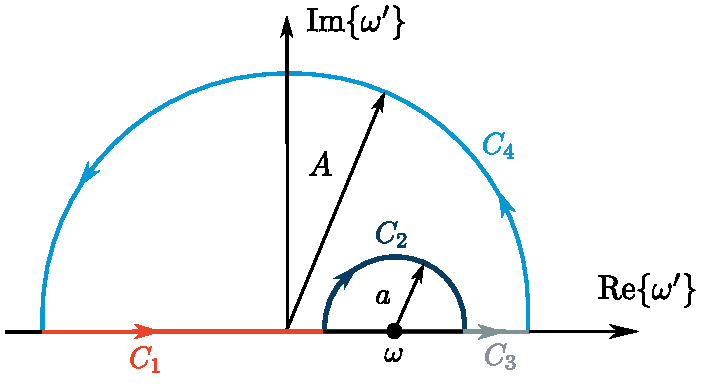
\includegraphics[width=8cm]{../../Figuras/integration.pdf}
	\caption{Contorno de integración $C$ conformado por cuatro curvas.}
	\label{integration_contour}
\end{figure}
%
Así, la Ec. \eqref{eq:Cauchy} se reescribe como
\begin{align*}
	\int_A^{\omega-a}\frac{[\varepsilon(\Omega)/\varepsilon_0-1]}{\Omega-\omega}\dd{\Omega}&+	\int_{\omega+a}^{A}\frac{[\varepsilon(\Omega)/\varepsilon_0-1])}{\Omega-\omega}\dd{\Omega}+\\
	&+	\int_0^{\pi}\frac{iA\;e^{i\Omega}\; [\varepsilon(A\;e^{i\Omega})/\varepsilon_0-1]}{A\;e^{i\Omega}-\omega}\dd{\Omega}-\int_0^{\pi}i\;[\varepsilon(\omega-ae^{-i\Omega})/\varepsilon_0-1]\dd{\Omega}=0.
\end{align*}
Integrando por partes la Ec. \eqref{seq:G}, se obtiene  
%
\begin{equation*}
	\frac{\varepsilon(\omega)}{\varepsilon_0}-1=\frac{i G(0)}{\omega}-\frac{ G'(0)}{\omega^2}+\frac{i G''(0)}{\omega^3}+...,
\end{equation*}
%
donde se empleó que $G(\tau)\rightarrow 0$ cuando $\tau\rightarrow \infty$. Además, dado que $G(\tau)$ es causal, $G(0)=0$; por lo que el primer término se anula al igual que los términos que decaen más rápido que $1/\omega^2$ a frecuencias altas. Con ello, por el lema de Jordan\footnote{El lema de Jordan establece que }, la integral sobre el segmento $C_4$ es 0 \cite{bohrenAbsorptionScatteringLight2008}. Por otro lado, al considerar el límite de $a\to 0$, la integral sobre $C_2$ es $i\pi[\varepsilon(\Omega)/\varepsilon_0-1]$ \cite{jacksonClassicalElectrodynamics2021a}. Finalmente, las integrales sobre los segmentos $C_1$ y $C_3$ equivalen a 
%
\begin{equation}
		\int_A^{\omega-a}\frac{[\varepsilon(\Omega)/\varepsilon_0-1]}{\Omega-\omega}\dd{\Omega}+	\int_{\omega+a}^{A}\frac{[\varepsilon(\Omega)/\varepsilon_0-1])}{\Omega-\omega}\dd{\Omega}=\text{PV}\int_{-\infty}^{\infty}\frac{[\varepsilon(\Omega)/\varepsilon_0-1]}{\Omega-\omega} \dd{\Omega}
\end{equation}
%
donde P.V. denota el valor principal de la integral \cite{arfkenMathematicalMethodsPhysicists2011a}. Por lo tanto, se obtiene 
%
\begin{equation}
	\PV{\int_{-\infty}^{\infty}\frac{[\varepsilon(\omega')/\varepsilon_0-1]}{\omega'-\omega} \dd{\omega'}}=i\pi[\varepsilon(\omega')/\varepsilon_0-1].
	\label{eq:KK_compleja}
\end{equation}
%
 Al separar la Ec. \eqref{eq:KK_compleja} en parte real e imaginaria, se obtienen las relaciones de Kramers-Kronig
%
\begin{align}
	\frac{\varepsilon'(\omega)}{\varepsilon_0}&=1+\frac{1}{\pi}\,\PV{\int_{-\infty}^{\infty}\frac{\varepsilon''(\omega')/\varepsilon_0}{\omega'-\omega}\dd{\omega'}} \label{seq:ReKK_inf}\\
	\frac{\varepsilon''(\omega)}{\varepsilon_0}&=-\frac{1}{\pi}\,\PV{\int_{-\infty}^{\infty}\frac{[\varepsilon'(\omega')/\varepsilon_0-1]}{\omega'-\omega}\dd{\omega'}}.\label{seq:ImKK_inf}
\end{align}
Dada la Ec. \eqref{seq:G}, se deduce que $\varepsilon(-\omega)/\varepsilon_0=\varepsilon^*(\omega^*)/\varepsilon_0$. Esta propiedad de simetría permite reescribir las Ecs. \eqref{seq:ReKK_inf} y \eqref{seq:ImKK_inf} en frecuencias positivas como
\begin{subequations}%
	\begin{tcolorbox}[
		ams align, breakable]
		\frac{\varepsilon'(\omega)}{\varepsilon_0}&=1+\frac{2}{\pi}\,\PV{\int_{0}^{\infty}\frac{\varepsilon''(\omega')/\varepsilon_0}{\omega'-\omega}\dd{\omega'}}\\ \label{seq:ReKK}
		\frac{\varepsilon''(\omega)}{\varepsilon_0}&=-\frac{2\omega}{\pi}\,\PV{\int_{0}^{\infty}\frac{[\varepsilon'(\omega')/\varepsilon_0-1]}{\omega'-\omega}\dd{\omega'}}.
		\label{seq:ImKK}
	\end{tcolorbox}
\end{subequations}\vspace*{1em}
%










